\documentclass{beamer}

\usetheme{Madrid}
    \setbeamertemplate{navigation symbols}{}
    \setbeamertemplate{caption}{\raggedright\insertcaption\par}
    \setbeamertemplate{footline}{}

\usepackage[brazil]{babel}
\usepackage[utf8]{inputenc}
\usepackage{color}
\usepackage{graphicx}
\usepackage{amsmath}

\title{A duração esperada da aposentadoria para homens no Brasil: 1980 -- 2025}


\author{Matheus Lobo Alves Ferreira}

\institute[UFMG]

\date{14 de dezembro de 2015}

\begin{document}
    
\begin{frame}[plain]
  \titlepage
\end{frame}

\begin{frame}{Contextualização}
	\begin{itemize}
		\item{Envelhecimento populacional }
		\item{Desequilíbrio dos programas de transferência de renda para idosos no mundo}
		\item{Programas são geralmente estruturados em Repartição Simples}
		Eu
		\item{No Brasil, gastos com o RGPS corresponderam a 14\% do PIB em 2005}
		\item{Regras de acesso aos benefícios incentivam a aposentadoria precoce}
		\item{Tendências recentes da dinâmica demográfica e do mercado de trabalho impactam diretamente o regime}
	\end{itemize}
\end{frame}

\begin{frame}{A dinâmica demográfica brasileira}
	\begin{itemize}
		\item{Transição demográfica: queda das taxas de mortalidade e fecundidade}
		\item{Redução da base de financiamento do RGPS}
		\item{Razão entre beneficiários e contribuintes estimada em 1,23 para 2050}
	\end{itemize}
	\begin{columns}[c]
	\column{6cm}
	\begin{figure}
		\caption{Brasil 1970}
		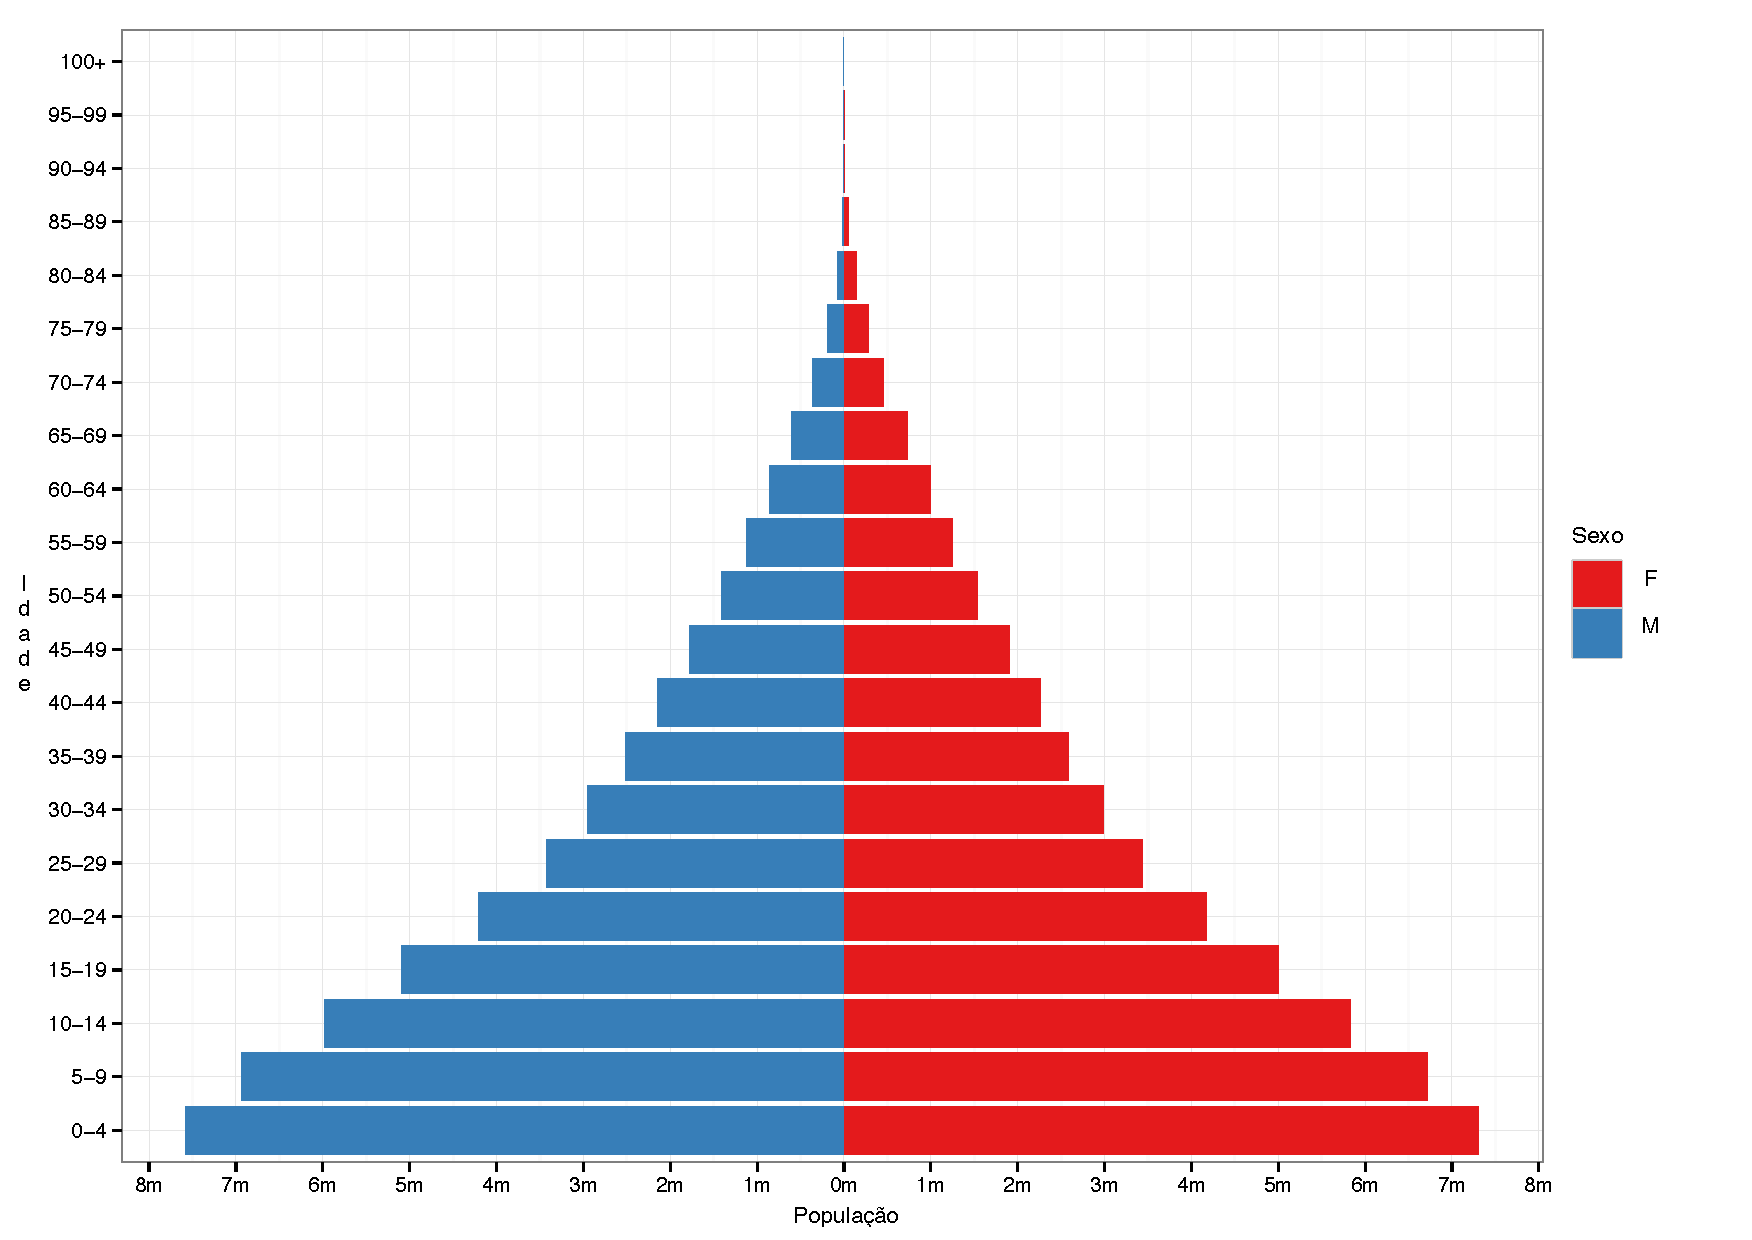
\includegraphics[width=\textwidth]{Graphs/1970.pdf}
	\end{figure}
	\column{6cm}
	\begin{figure}
		\caption{Brasil 2050}
		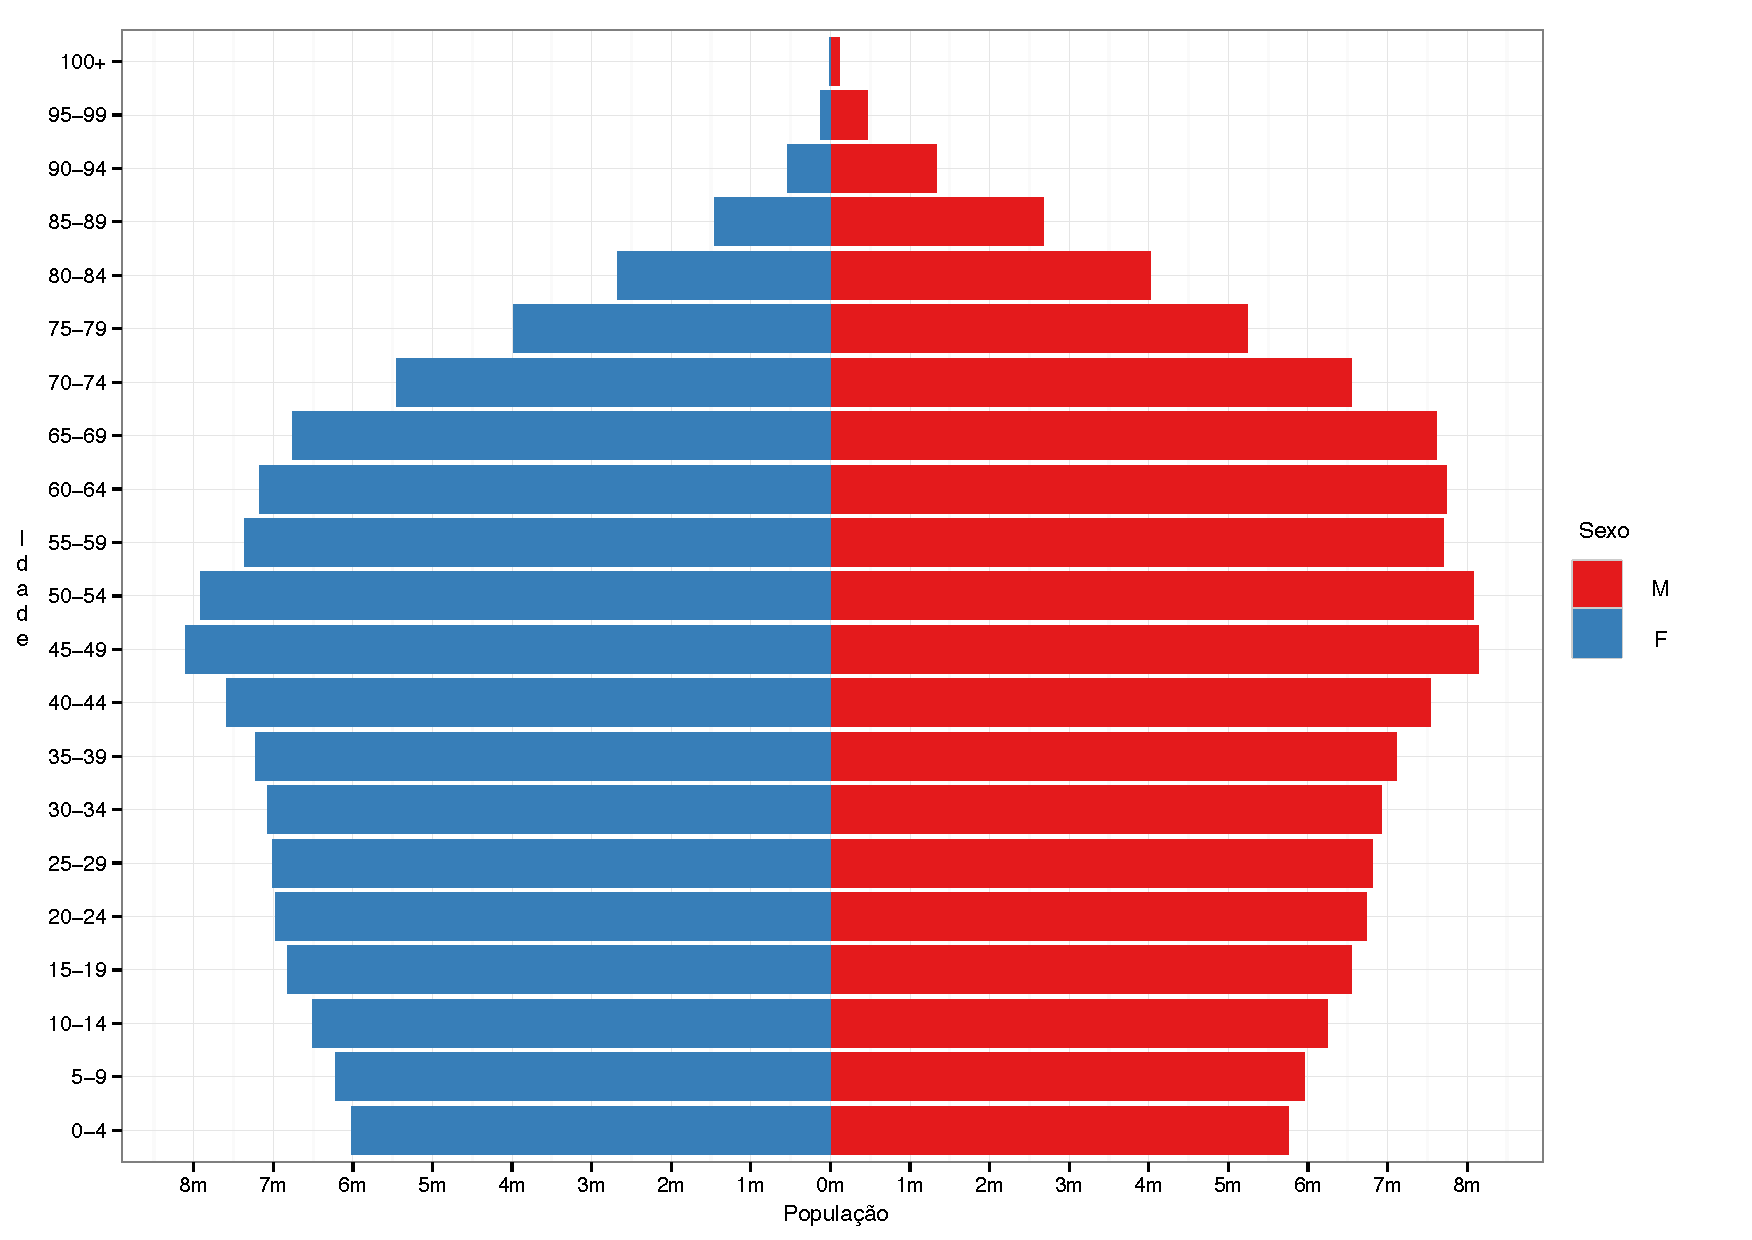
\includegraphics[width=\textwidth]{Graphs/2050.pdf}
	\end{figure}
	\end{columns}
\end{frame}

\begin{frame}{Mercado de trabalho no Brasil}
Mudanças Recentes:
	\begin{itemize}
		\item{Aumento da taxa de atividade feminina}
		\item{Queda da taxa de atividade masculina}
	\end{itemize}
Apesar das mudanças observadas, o MPS assume que a taxa de atividade permanece constante em suas projeções. 
	\begin{itemize}
		\item{Uso do modelo Lee--Carter para projetar a taxa de atividade masculina}
		\item{Dificuldade para projetar a taxa de atividade feminina}
	\end{itemize}
\end{frame}

\begin{frame}{Dados e Métodos}
Fontes de dados:
	\begin{itemize}
		\item{Latin America Human Mortality Database\footnote{http://www.lamortalidad.org/} (1980 -- 2010)}
		\item{Pesquisa Nacional por Amostra de Domicílio -- PNAD (1980 -- 2013)}
	\end{itemize}	
Métodos:
	\begin{itemize}
		\item{Correção de Subregistro de Óbitos} 
		\item{Interpolação das taxas de mortalidade (P-Splines)}
		\item{Suavização das taxas de atividade (LOESS)}
	\end{itemize}
\end{frame}

\begin{frame}{Dados e Métodos}
	\begin{figure}[!htb]
		\caption{Superfície de Mortalidade: Brasil 1980 - 2010}
		\begin{center}
			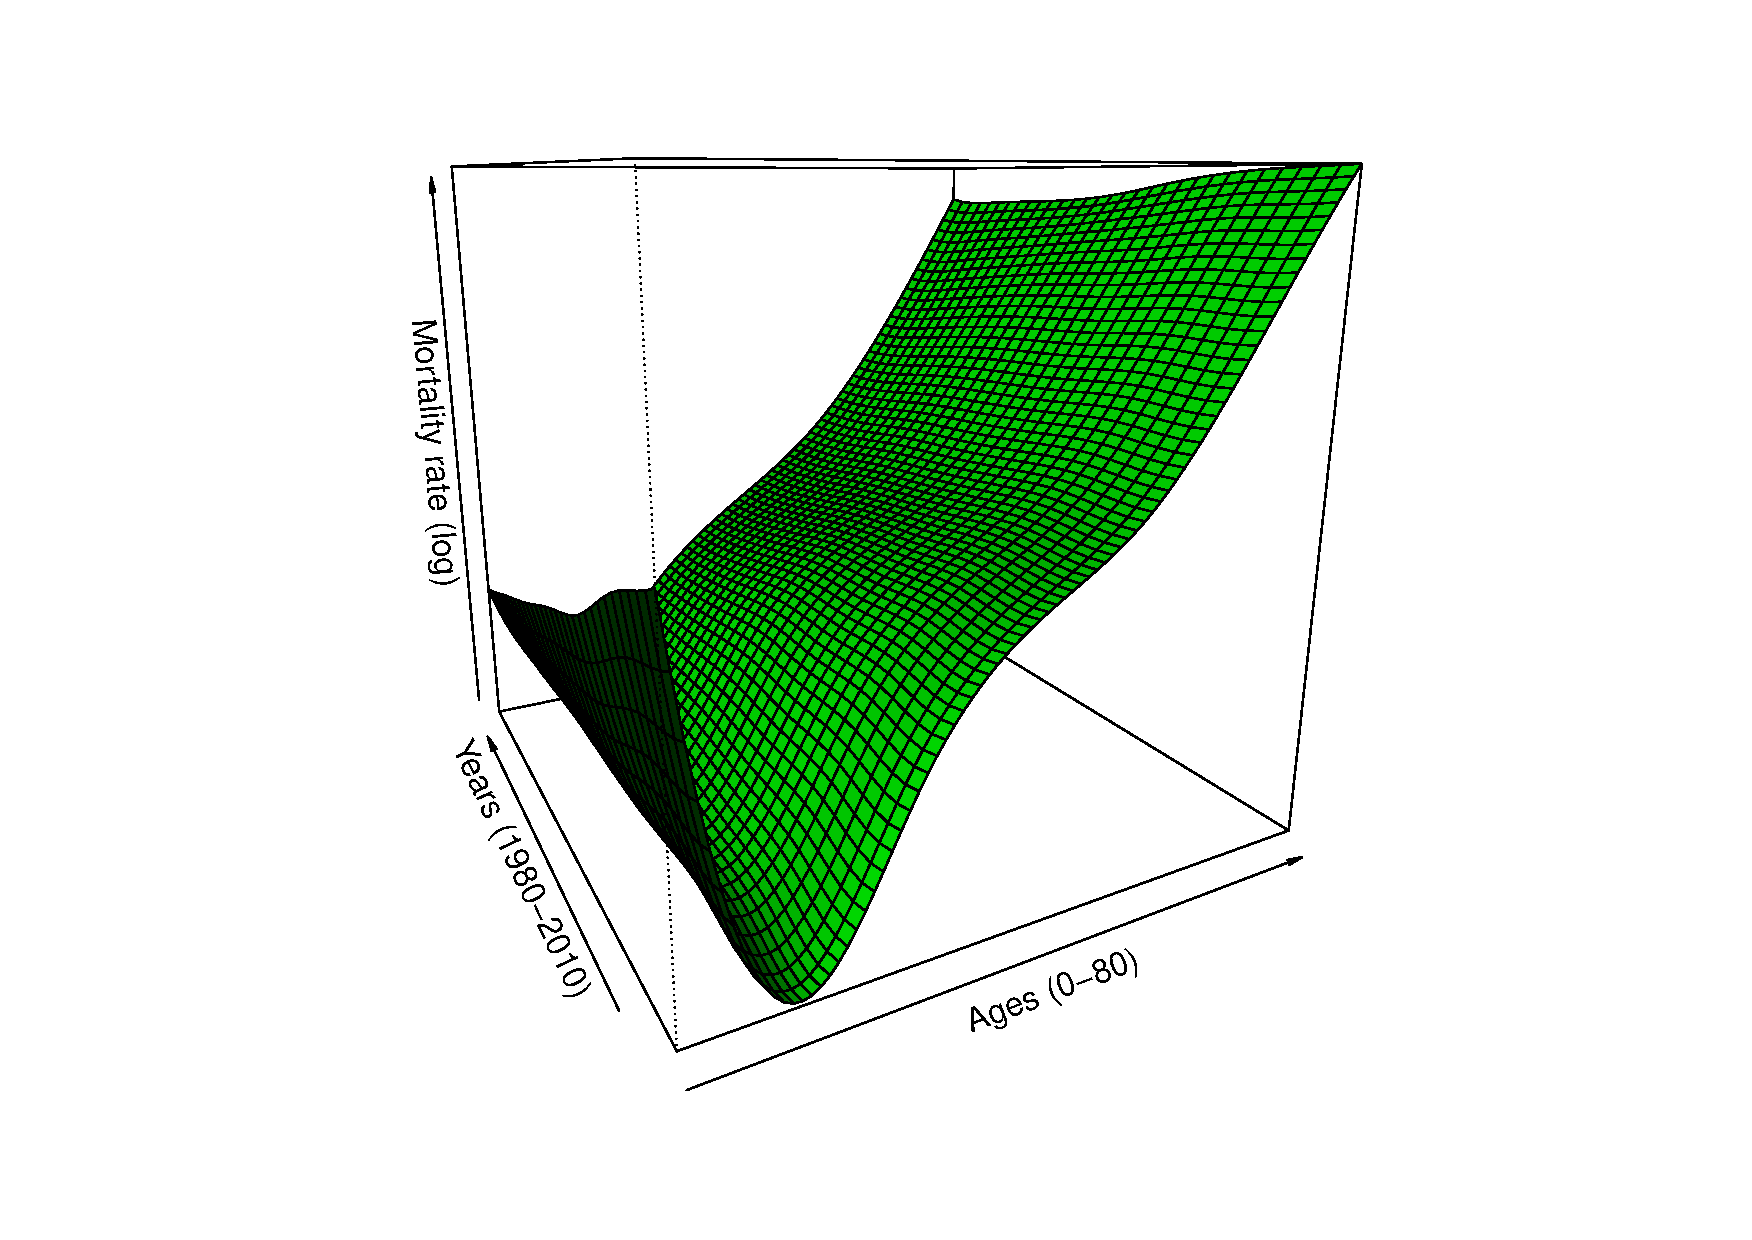
\includegraphics[scale = 0.3]{Graphs/MortalitySurface.pdf}
		\end{center}
	\end{figure} 
\end{frame}



\begin{frame}{Lee--Carter}
	\begin{itemize}
		\item{Modelo amplamente aplicado em demografia e atuária como um modelo estocástico para projeção de taxas de mortalidade}
		\item{Uso do modelo para projetar a taxa de atividade}
		\item{Modelo parcimonioso -- apenas três parâmetros estimados}
	\end{itemize} 
	\begin{equation}
  		ln(m_{x,t}) = a_{x}+b_{x}k_{t} + \epsilon_{x,t}
	\end{equation}
	\begin{equation}
  		ln(LFPR_{x,t}) = a_{x}+b_{x}k_{t} + \epsilon_{x,t}
	\end{equation}
	\begin{itemize}
		\item{$a$ -- perfil etário médio}
		\item{$k$ -- indica as mudanças no nível da taxa ao longo do tempo}
		\item{$b$ -- mostra o efeito da tendência de $k$ para cada grupo etário}
	\end{itemize}
\end{frame}

\begin{frame}{Lee--Carter}
	\begin{columns}[c]
	\column{6cm}
	\begin{figure}
		\caption{$a_{x}$ Taxa de Mortalidade}
		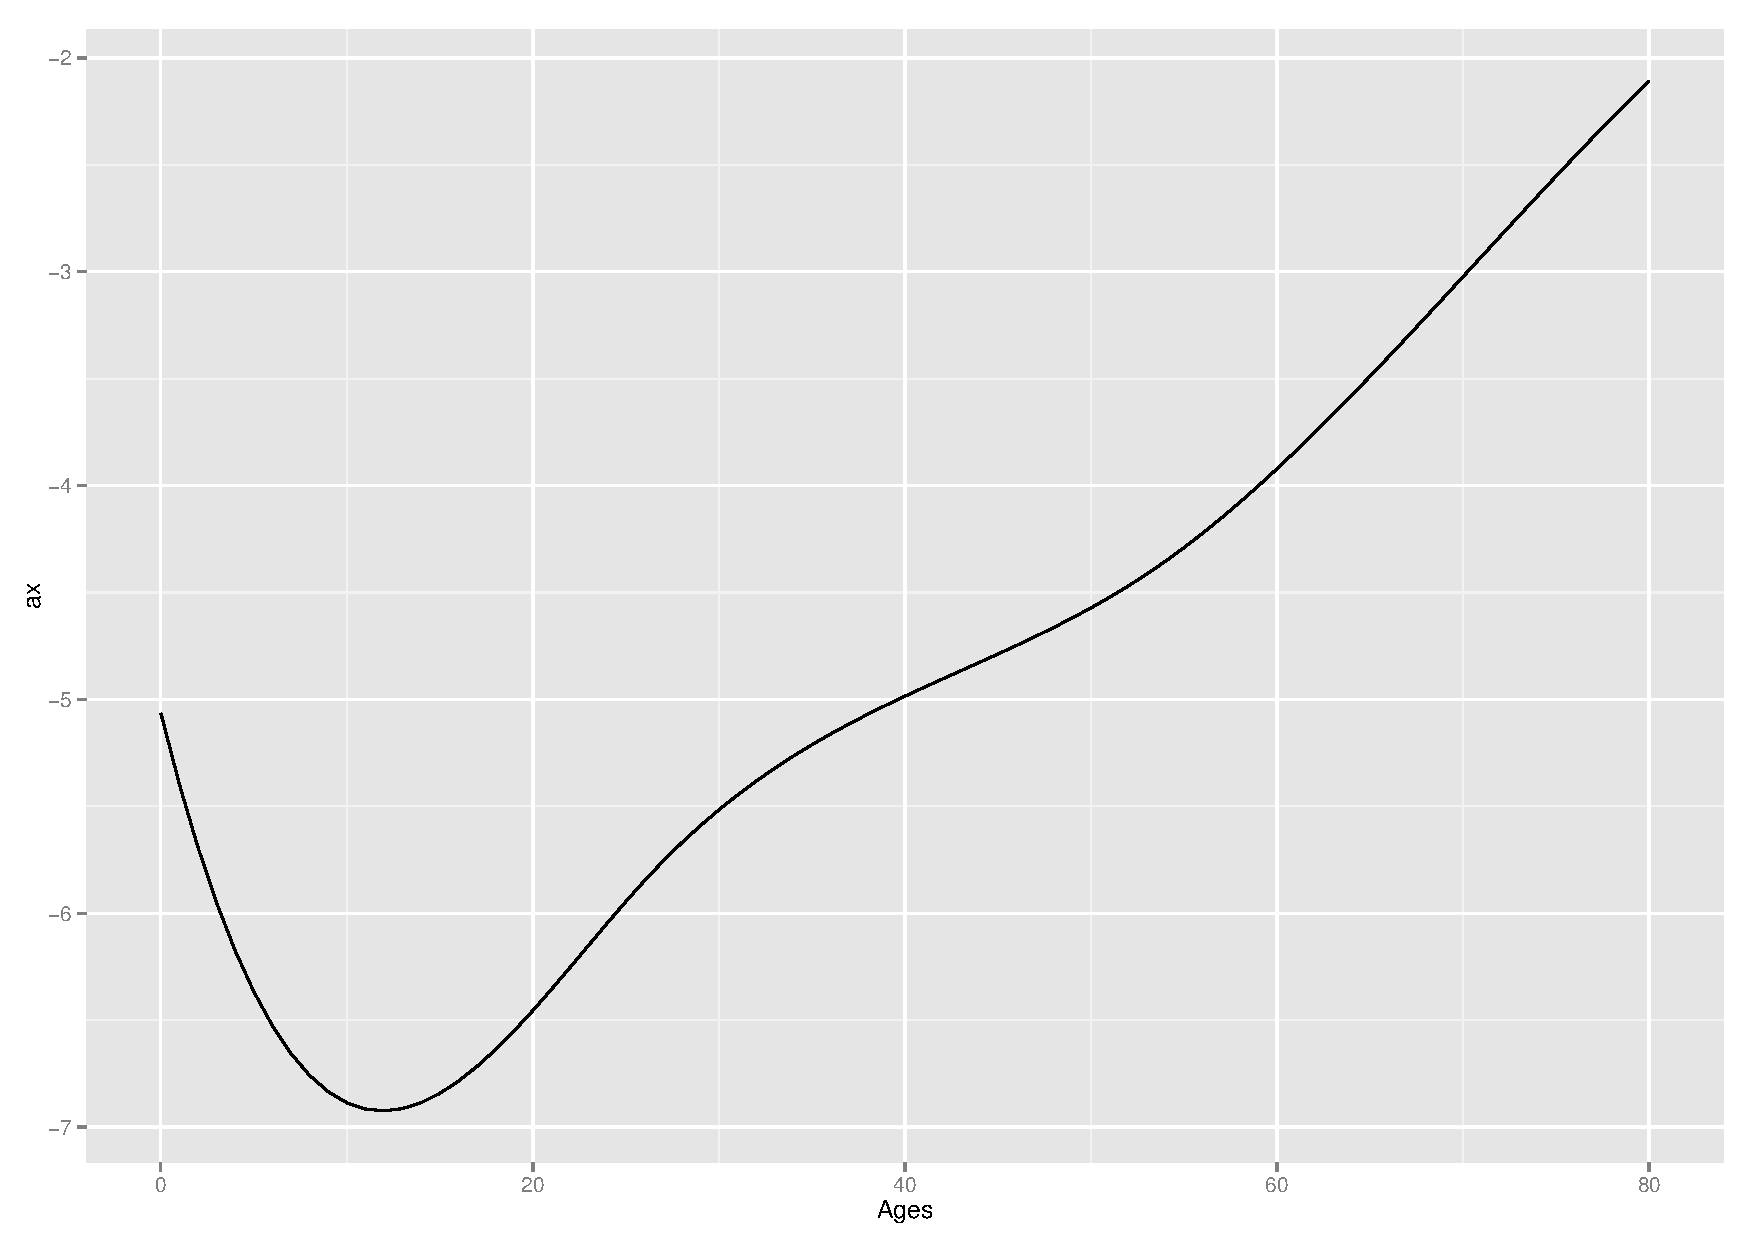
\includegraphics[width=\textwidth]{Graphs/DR_LC_ax.pdf}
	\end{figure}
	\column{6cm}
	\begin{figure}
		\caption{$a_{x}$ Taxa de Atividade}
		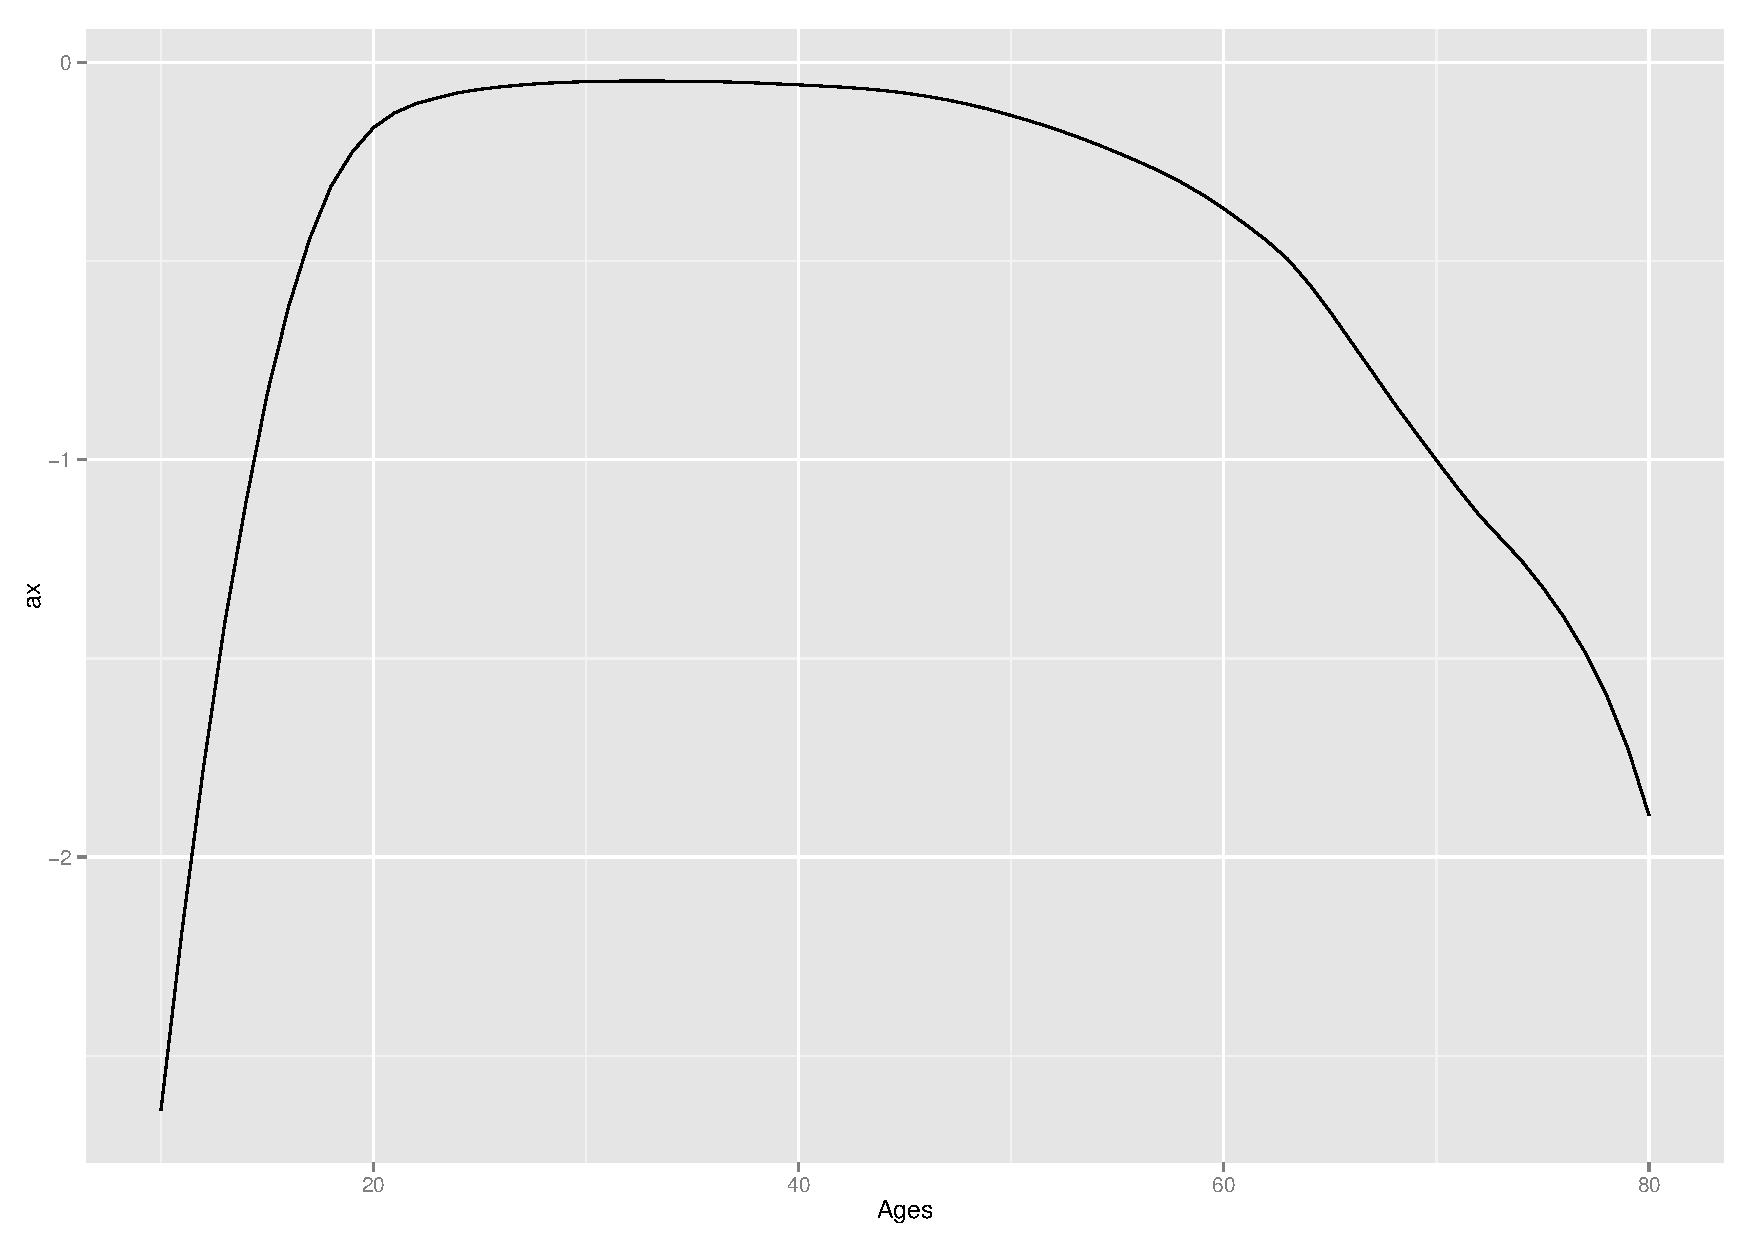
\includegraphics[width=\textwidth]{Graphs/LFPR_LC_ax.pdf}
	\end{figure}
	\end{columns}  
\end{frame}

\begin{frame}{Lee--Carter}
	\begin{columns}[c]
	\column{6cm}
	\begin{figure}
		\caption{$k_{t}$ Taxa de Mortalidade}
		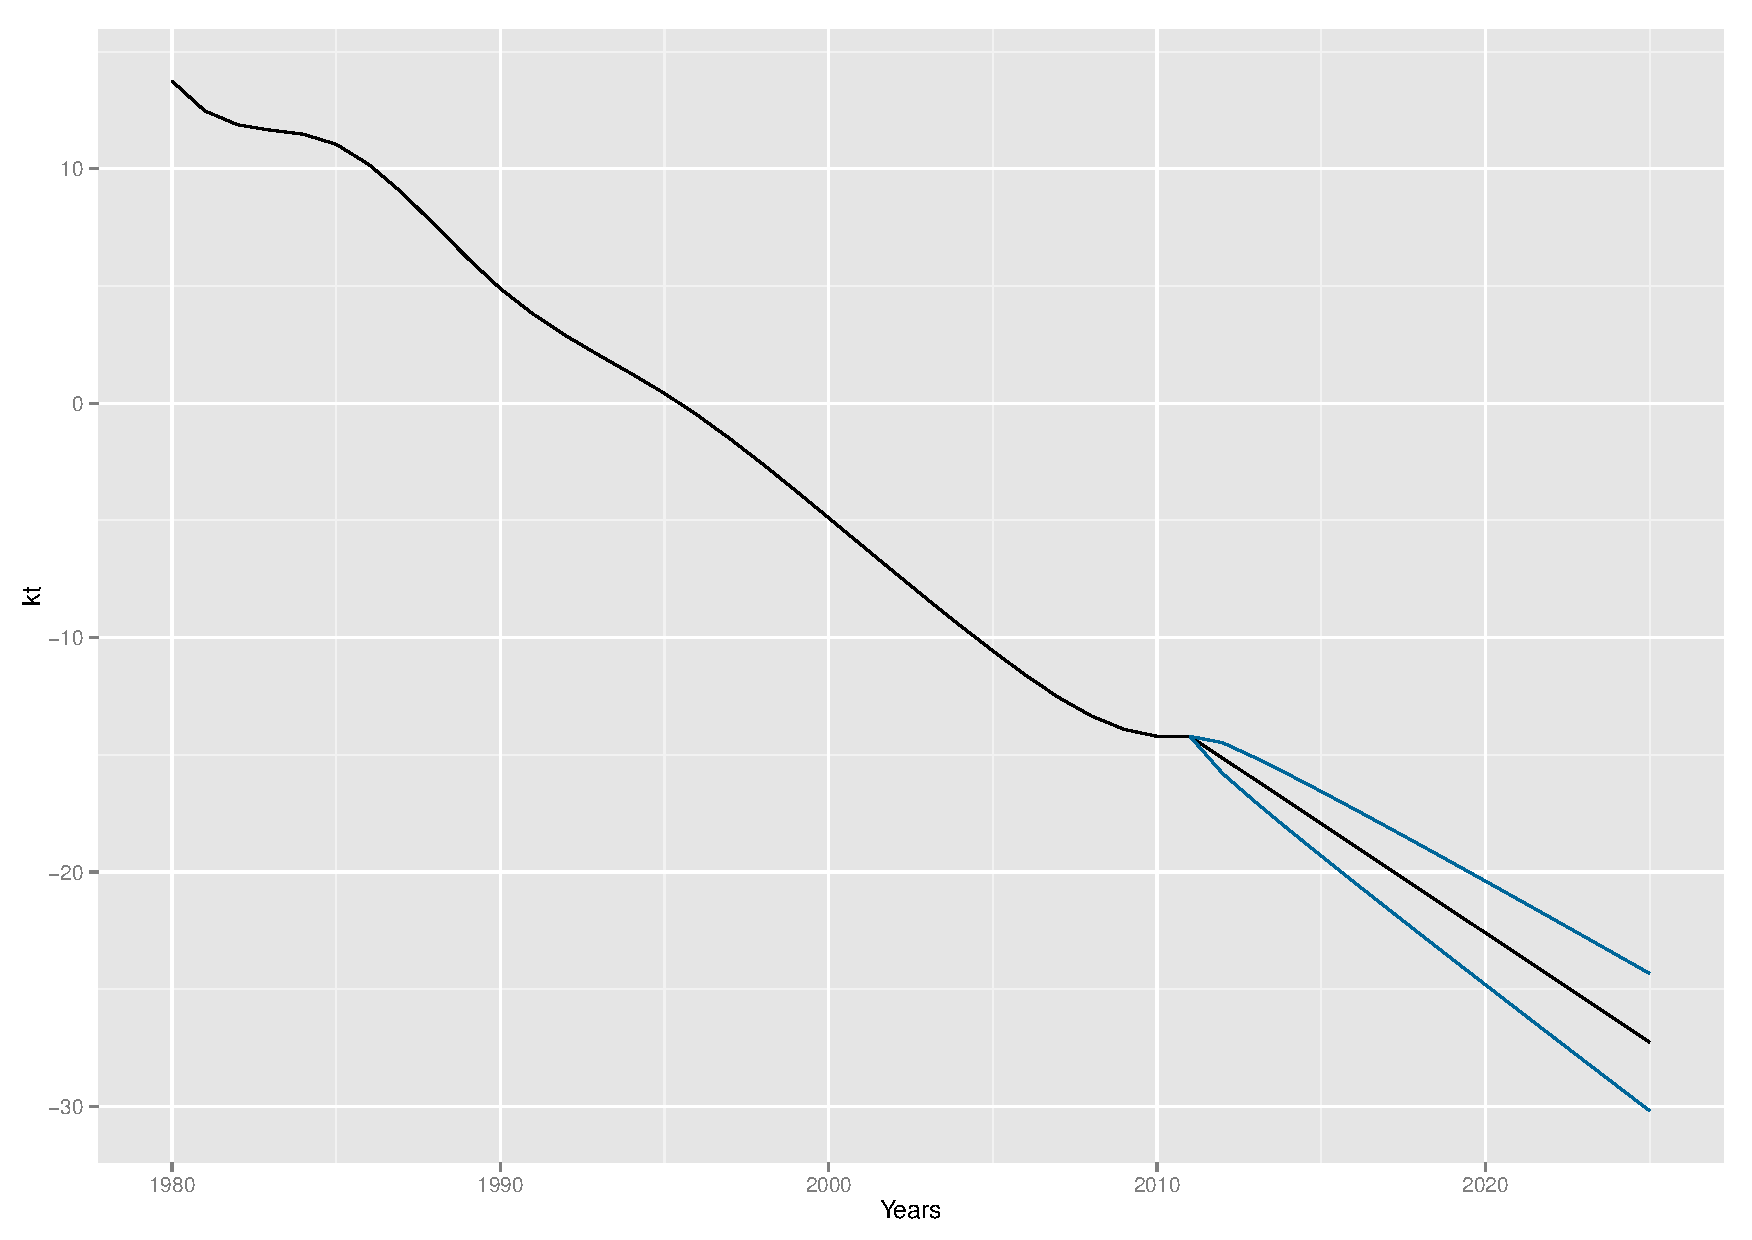
\includegraphics[width=\textwidth]{Graphs/DR_LC_kt_f.pdf}
	\end{figure}
	\column{6cm}
	\begin{figure}
		\caption{$k_{t}$ Taxa de Atividade}
		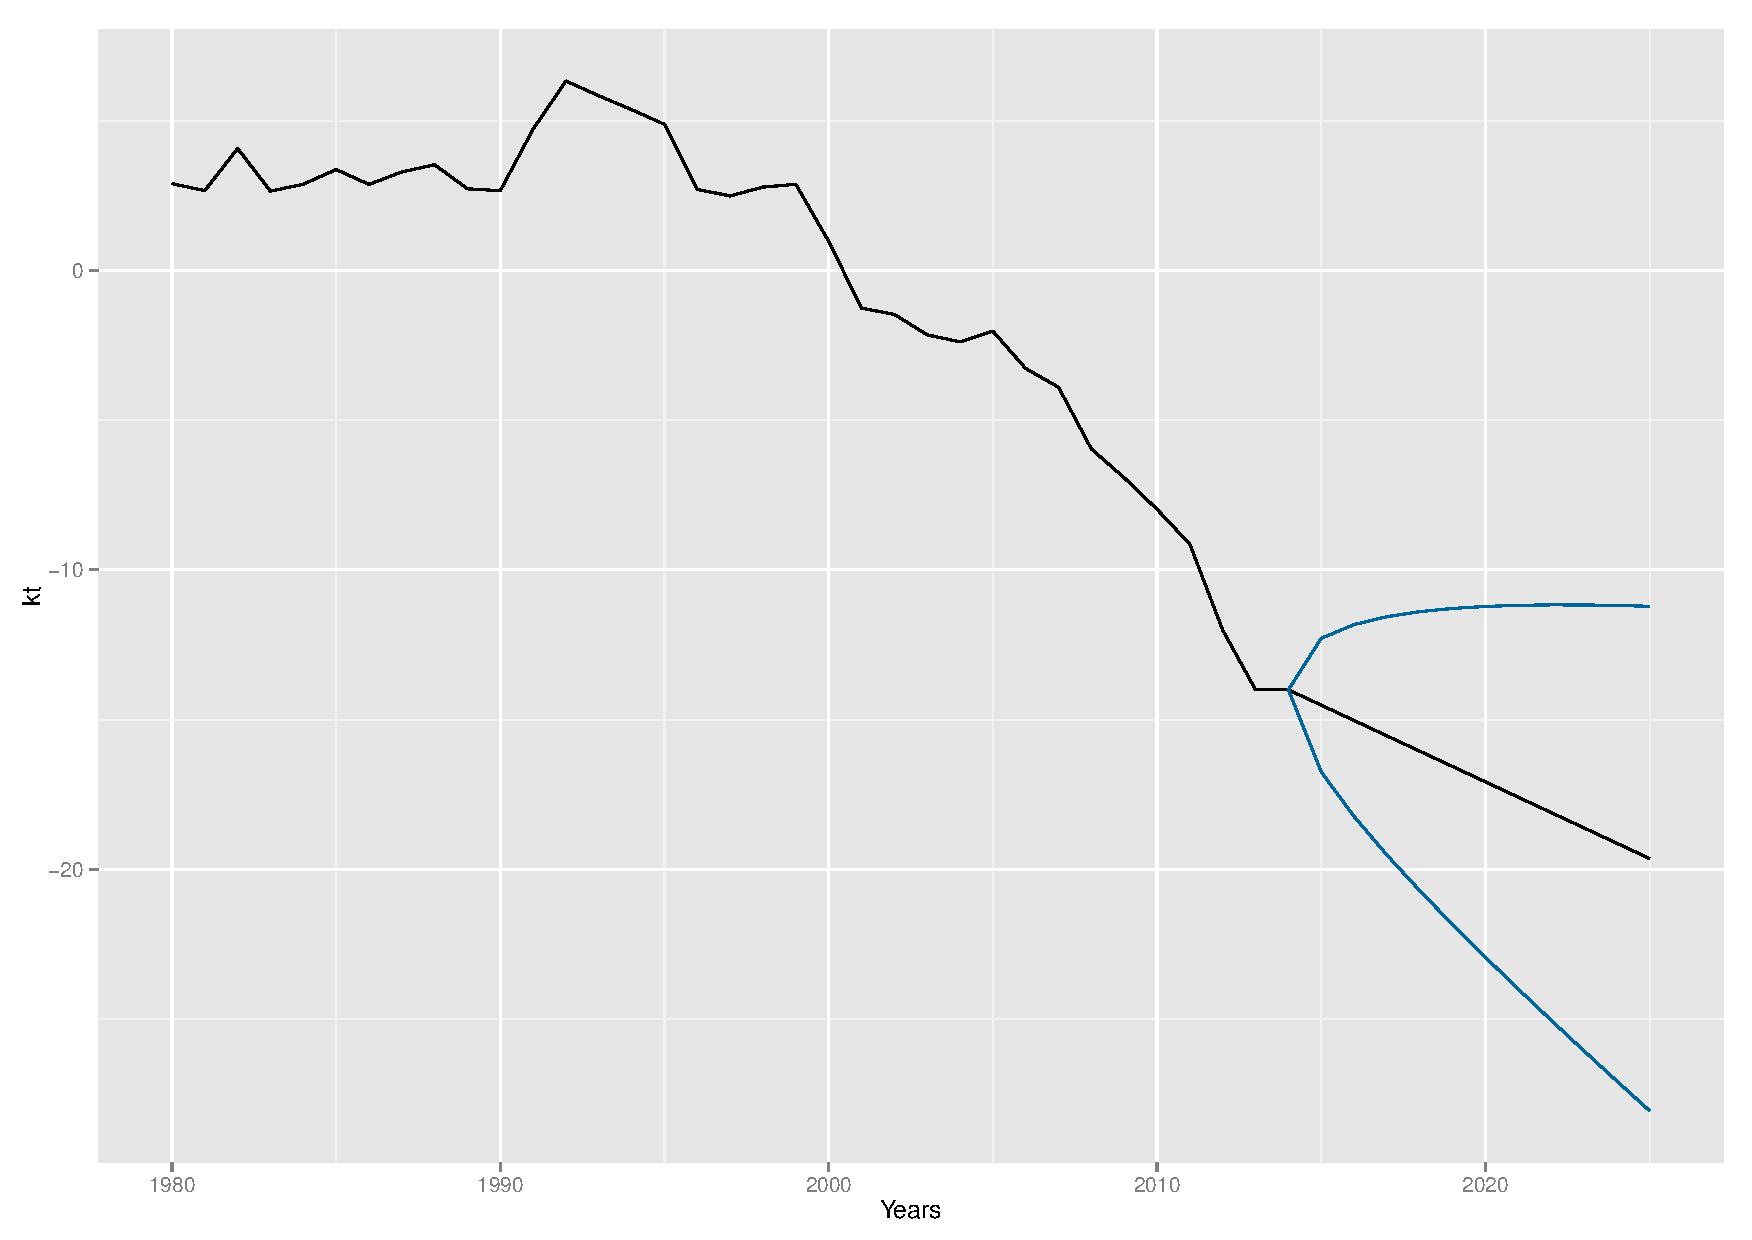
\includegraphics[width=\textwidth]{Graphs/LFPR_LC_kt_f.pdf}
	\end{figure}
	\end{columns}  
\end{frame}

\begin{frame}{Lee--Carter}
	\begin{columns}[c]
	\column{6cm}
	\begin{figure}
		\caption{$b_{x}$ Taxa de Mortalidade}
		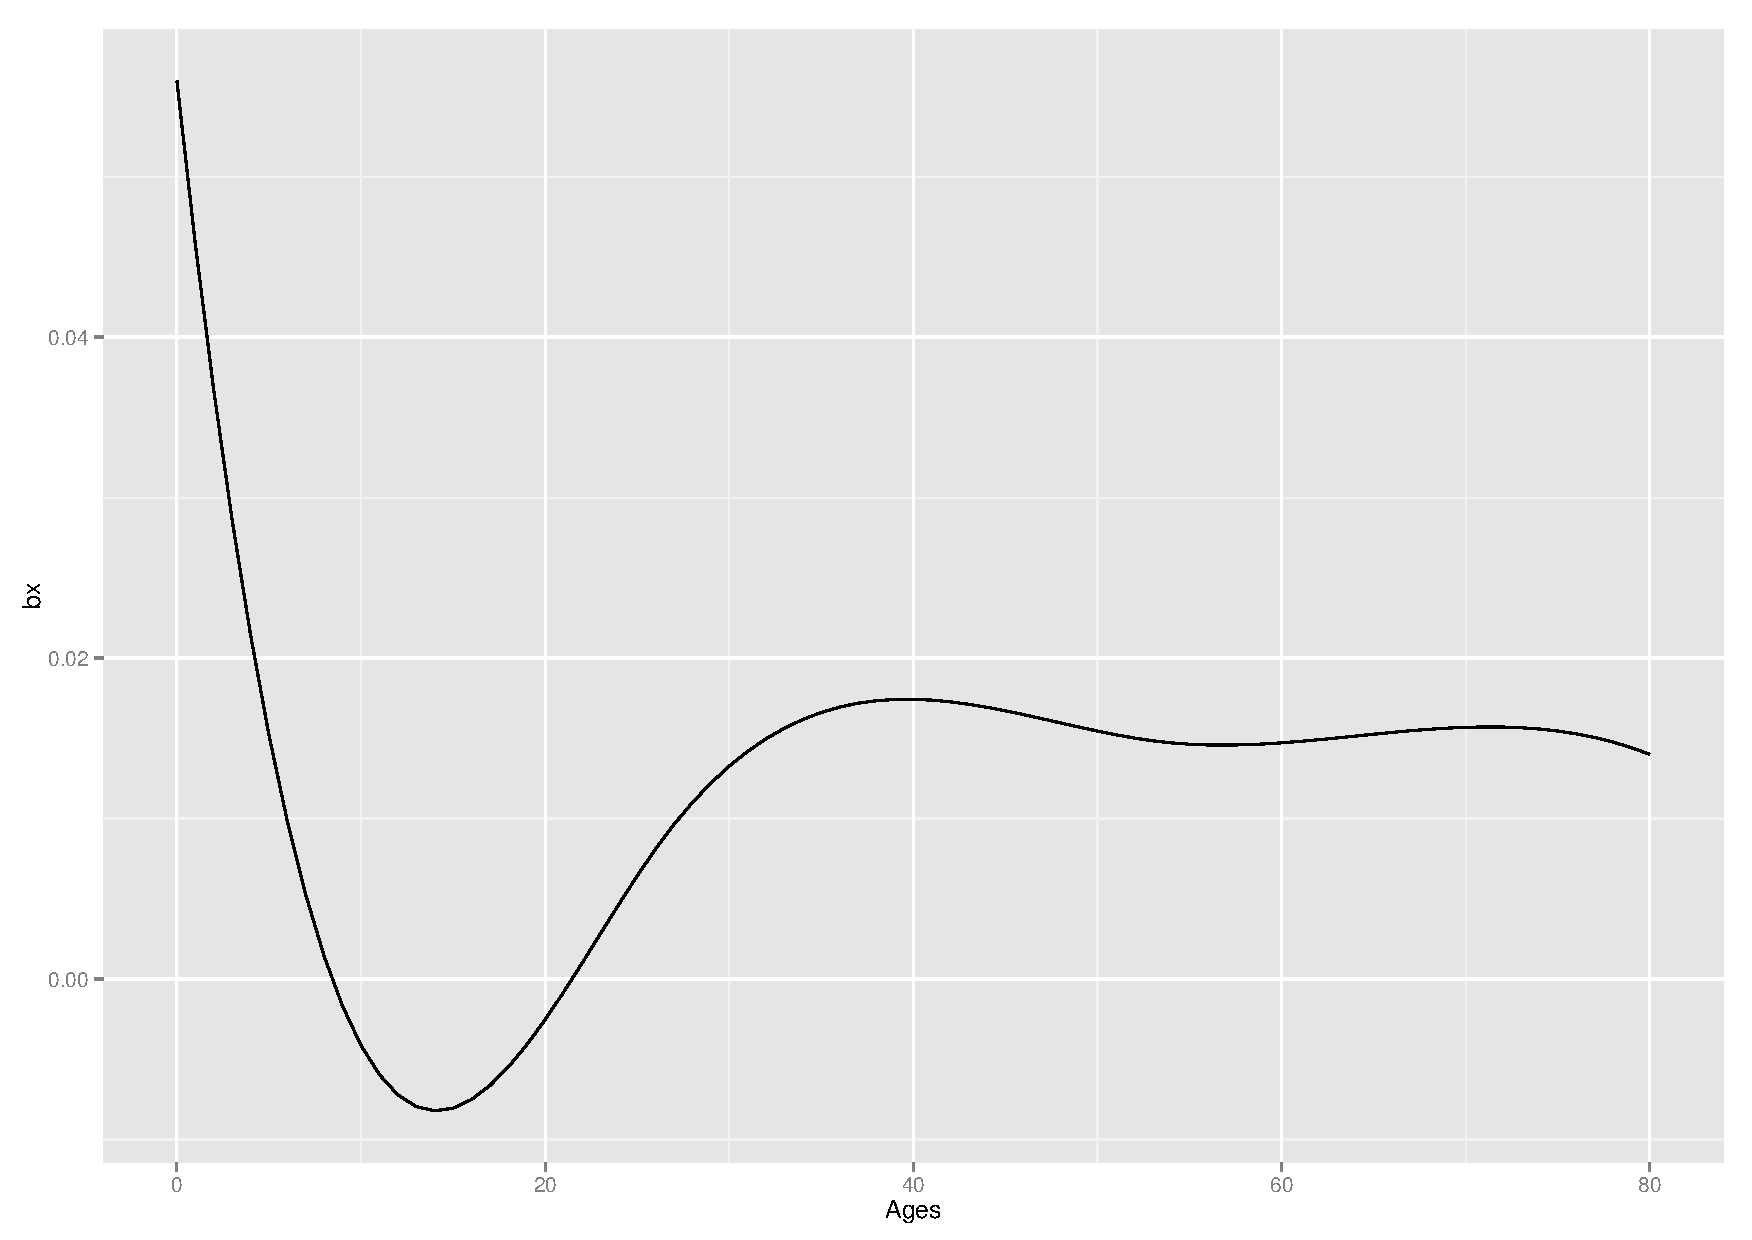
\includegraphics[width=\textwidth]{Graphs/DR_LC_bx.pdf}
	\end{figure}
	\column{6cm}
	\begin{figure}
		\caption{$b_{x}$ Taxa de Atividade}
		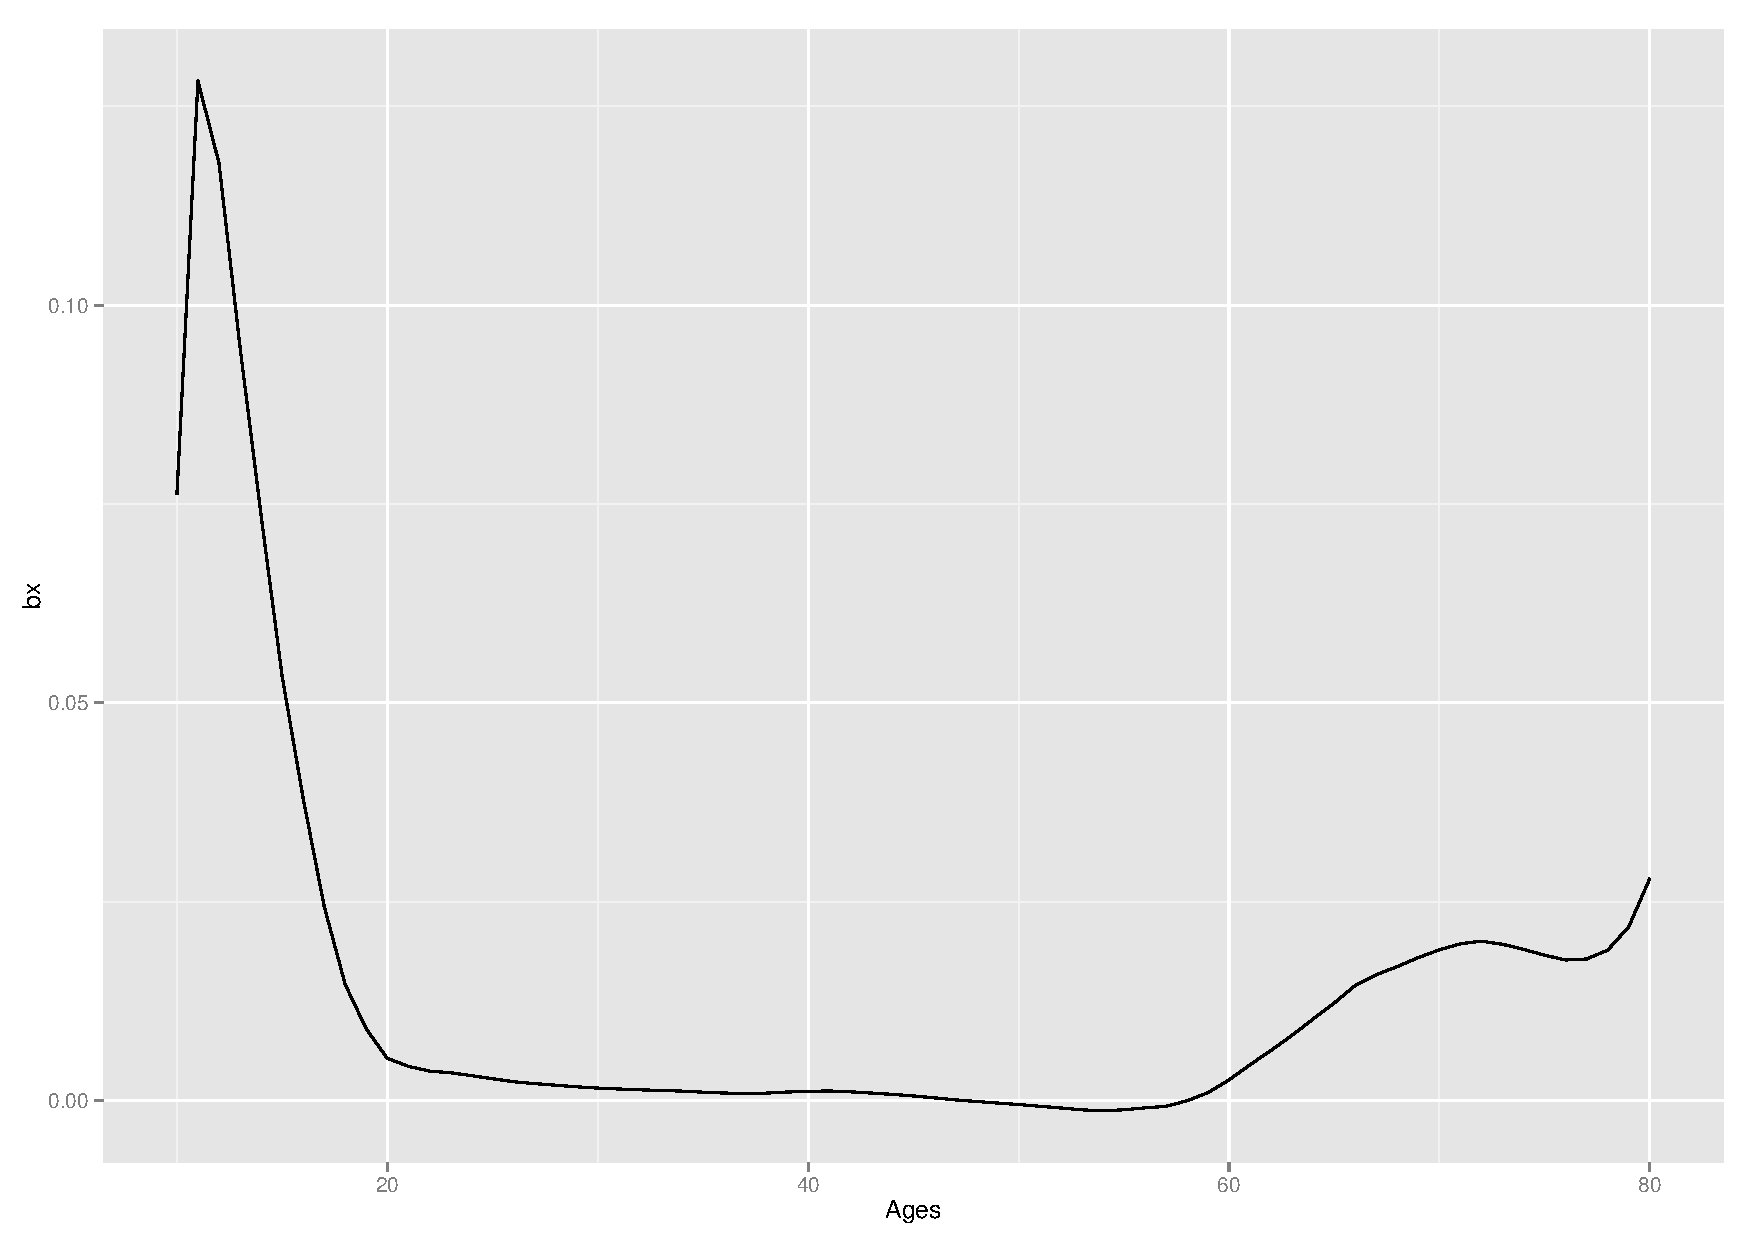
\includegraphics[width=\textwidth]{Graphs/LFPR_LC_bx.pdf}
	\end{figure}
	\end{columns}  
\end{frame}

\begin{frame}{Lee--Carter}
	\begin{columns}[c]
	\column{6cm}
	\begin{figure}
		\caption{LC Taxa de Mortalidade}
		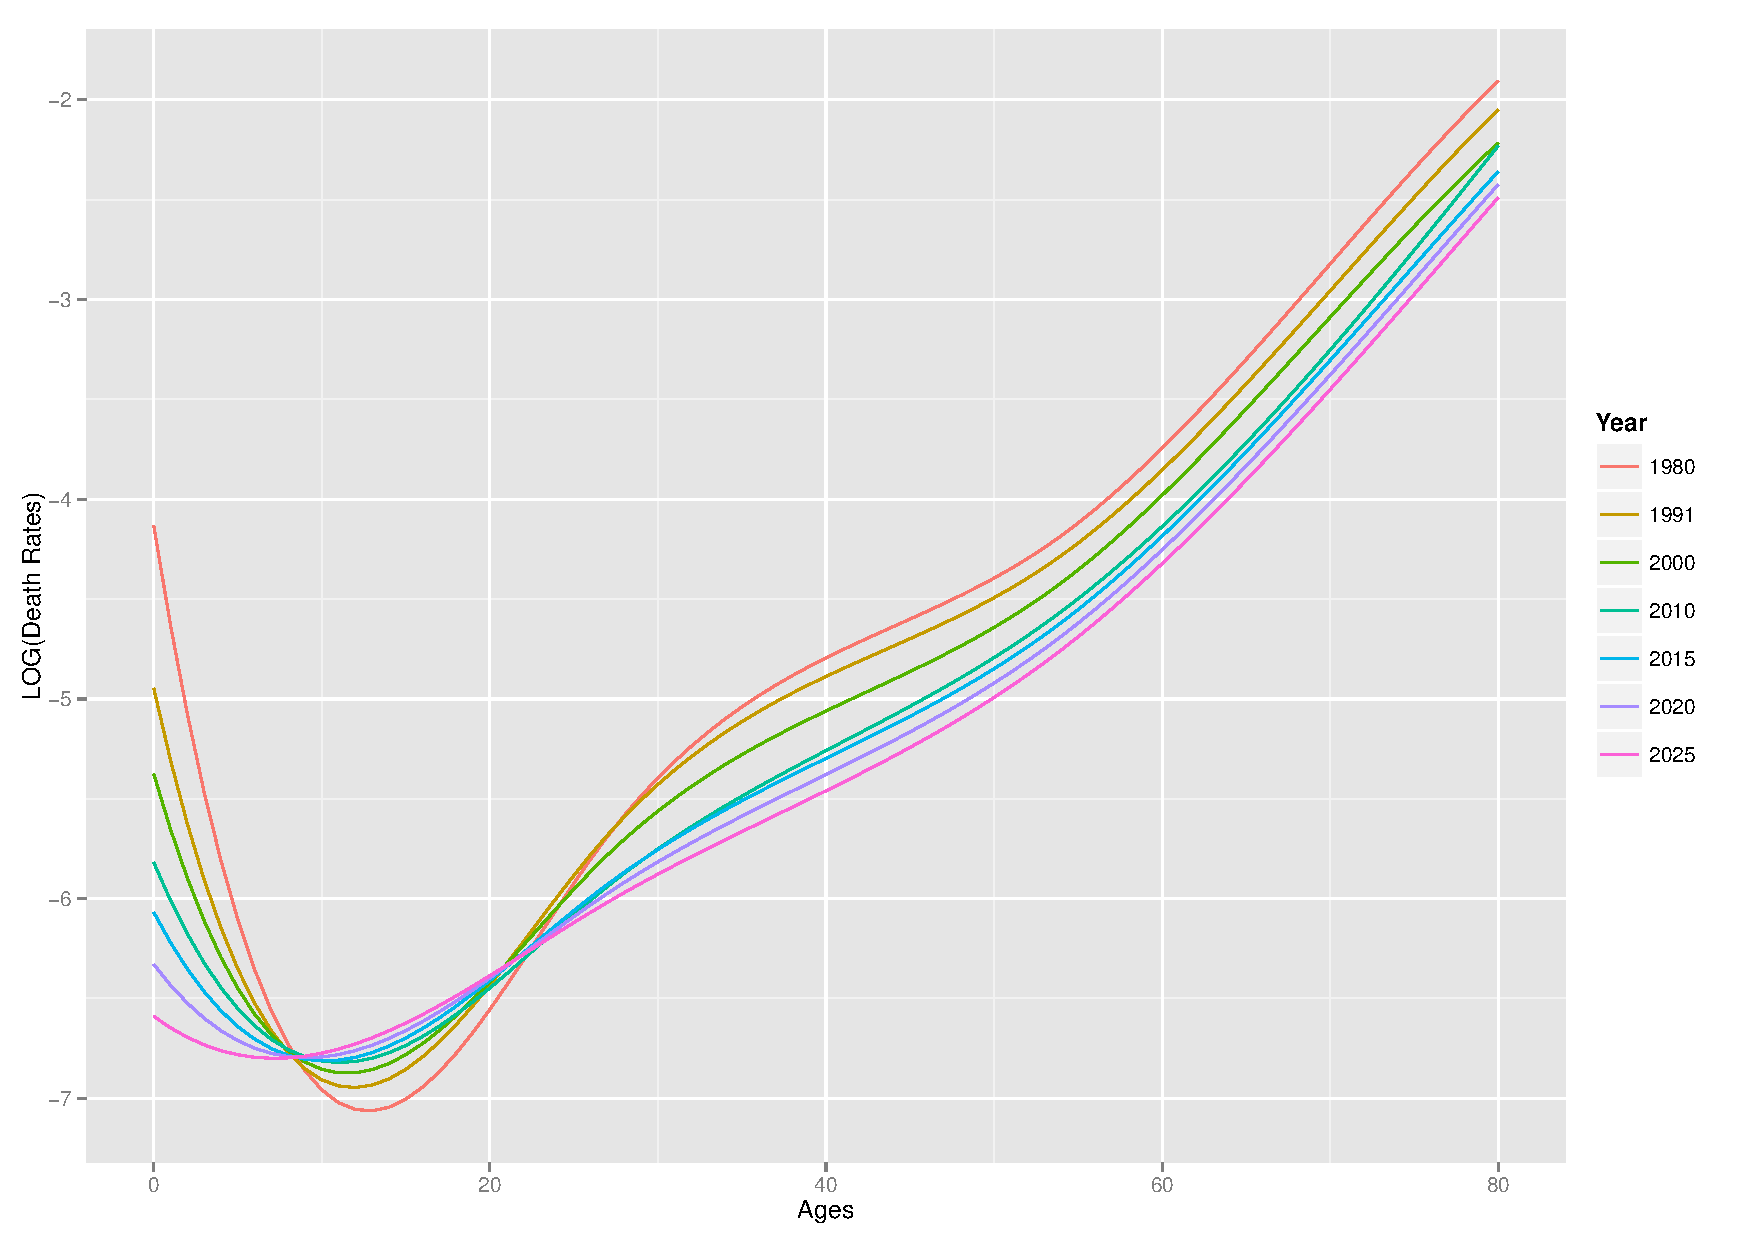
\includegraphics[width=\textwidth]{Graphs/DR_select.pdf}
	\end{figure}
	\column{6cm}
	\begin{figure}
		\caption{LC Taxa de Atividade}
		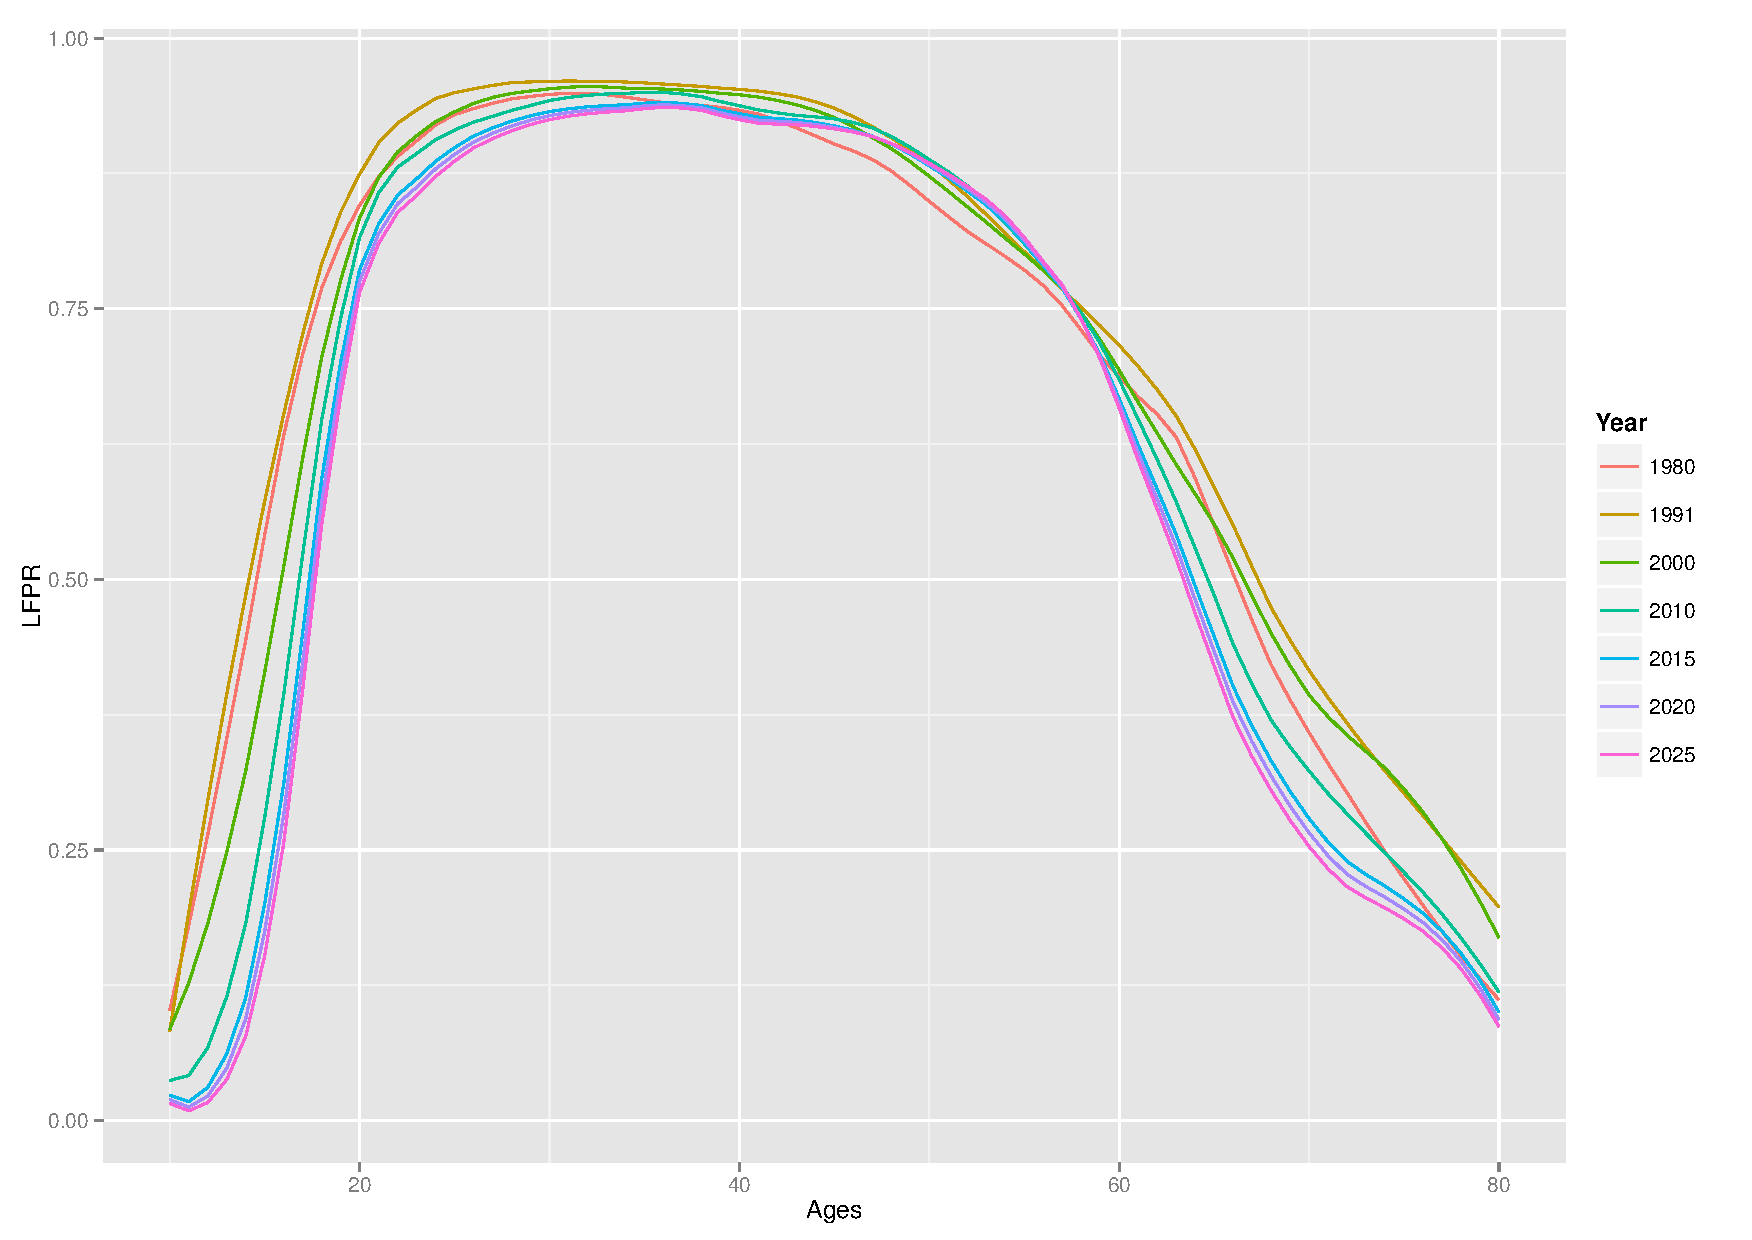
\includegraphics[width=\textwidth]{Graphs/LFPR_select.pdf}
	\end{figure}
	\end{columns}  
\end{frame}

\begin{frame}{Lee--Carter}
	\begin{columns}[c]
	\column{6cm}
	\begin{figure}
		\caption{Validação LC Mortalidade}
		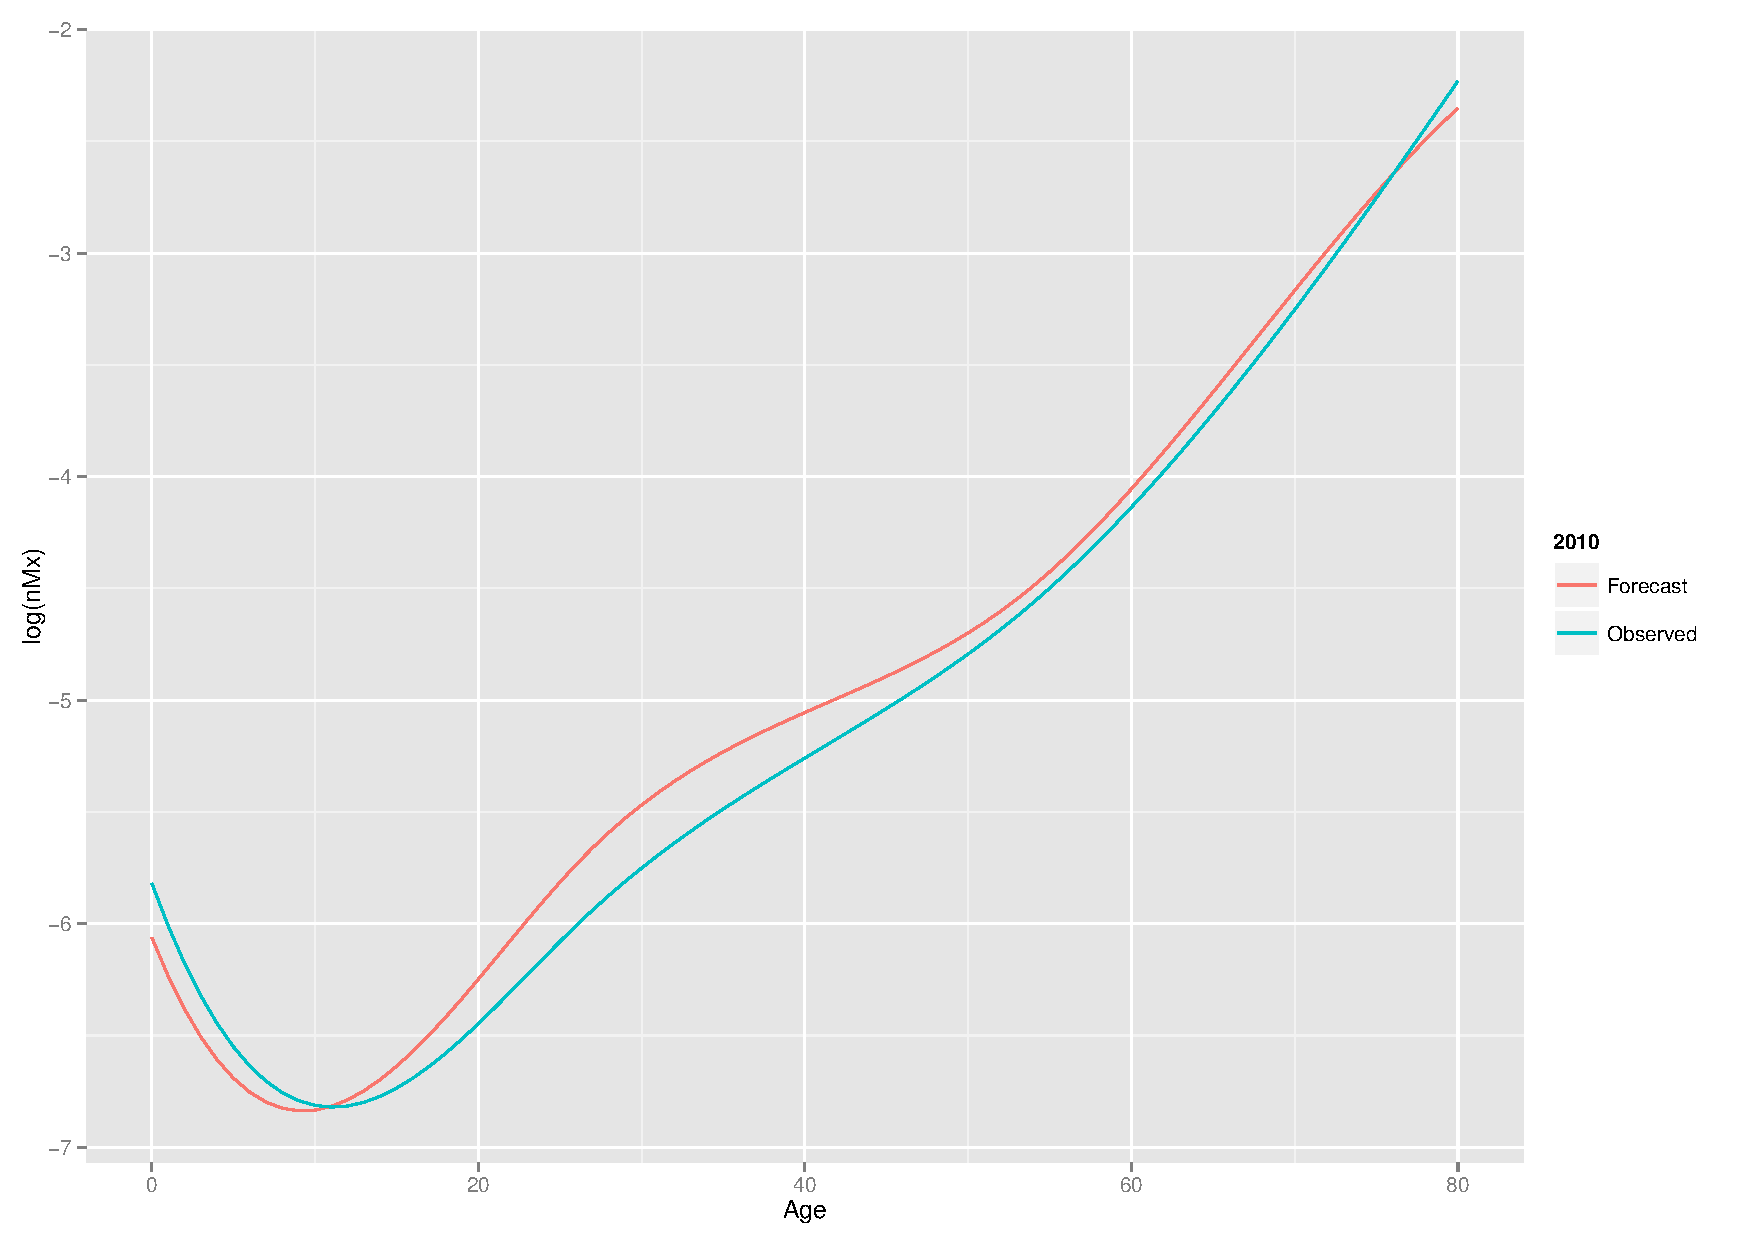
\includegraphics[width=\textwidth]{Graphs/DR_validation.pdf}
	\end{figure}
	\column{6cm}
	\begin{figure}
		\caption{Validação LC Taxa de Atividade}
		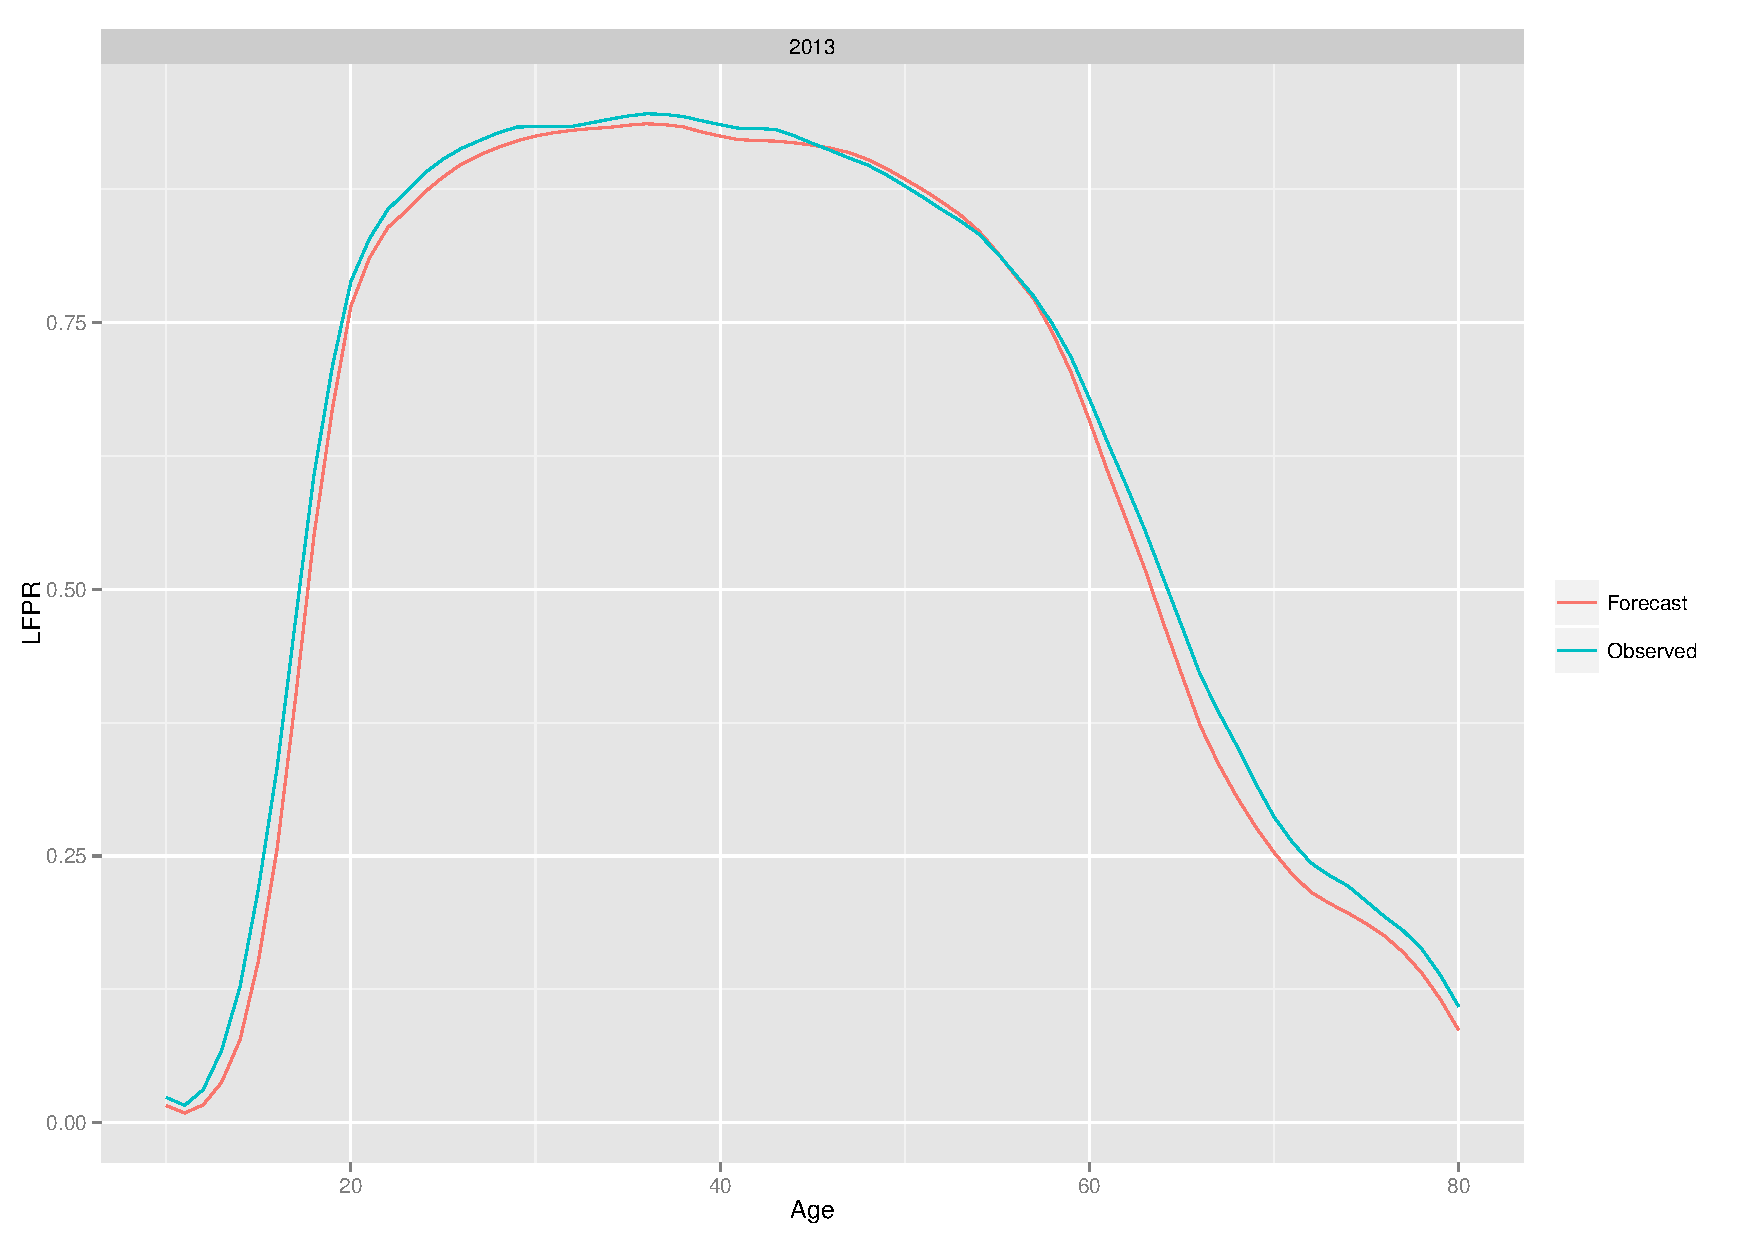
\includegraphics[width=\textwidth]{Graphs/LFPR_validation.pdf}
	\end{figure}
	\end{columns}  
\end{frame}

\begin{frame}{A duração esperada da aposentadoria - ELRP}
	\begin{itemize}
		\item{Entrada no mercado de trabalho ocorre em torno dos 20 anos}
		\item{Saída do marcado de trabalho começa por volta dos 50 anos}
		\item{A duração esperada da aposentadoria pode ser estimada através de uma média ponderada da expectativa de vida}
	\end{itemize}
	\begin{equation}
		ELRP = \rho^{20-50}\sum_{x=50}^{80}S_{x}T_{x}\gamma_{x}[1-(0,5q_x)]\left[\dfrac{(e_x + e_{x+1})}{2}\right]
	\end{equation}
	\begin{itemize}
		\item{$S_{x}$ -- probabilidade de permanecer vivo até a idade \emph{x}}
		\item{$T_{x}$ -- probabilidade de se manter no mercado de trabalho até a idade \emph{x}}
		\item{$\gamma_{x}$ -- probabilidade de se aposentar à idade \emph{x}}
		\item{$e_{x}$ -- expectativa de vida à idade \emph{x}}
	\end{itemize}
\end{frame}

\begin{frame}{Resultados}
	\begin{columns}[c]
	\column{0.5\textwidth}
	\begin{table}[!htb]
		\caption{ELRP -- Brasil}
		\begin{tabular}{cccc}
		Ano & ELRP & $e_{20}$ & $\tfrac{ELRP}{e_{20}}$ 
		\\
		\hline \hline
		1980 & 4,925 & 46,54 & 10,58                                    
		\\
		1991 & 5,498 & 47,95 & 11,47                                    
		\\
		2000 & 6,497 & 50,07 & 12,98                                   
		 \\
		2010 & 8,185 & 52,00 & 15,74                                   
		\\
		2015 & 9,052 & 53,02 & 17,07                                    
		\\
		2020 & 9,792 & 54,12 & 18,09                                    
		\\
		2025 & 10,570 & 55,26 & 19,13                                    
		\\ \hline \hline
		\end{tabular}
	\end{table}
	\column{0.5\textwidth}
	\begin{table}[htb]
		\caption{ELRP -- EUA}
		\label{tab3}
		\begin{tabular}{cccc}
		Ano & ELRP & $e_{20}$ & $\tfrac{ELRP}{e_{20}}$ 
		\\
		\hline \hline
		1870 & 0,83 & 41,14 & 2,1		
		\\
		1890 & 2,26 & 40,96 & 5,5		
		\\
		1910 & 3,38 & 41,73 & 7,9		
		\\
		1930 & 4,95 & 44,45 & 10,9	
		\\
		1950 & 6,68 & 46,77 & 13,6	
		\\
		1970 & 8,59 & 49,65 & 17,2	
		\\
		1990 & 12,66 & 52,95 & 23,8	
		\\ 
		\hline \hline
		\end{tabular}
	\end{table}
	\end{columns}
	\begin{itemize}
		\item{Aumento da ELRP no Brasil durante os próximos anos?}
		\item{Transição demográfica americana 1800--1940}
		\item{Transição demográfica brasileira 1950--...}
		\item{Redução da vida ativa dos homens brasileiros}
	\end{itemize}
\end{frame}

\begin{frame}{Conclusão}
Destaques:
	\begin{itemize}
		\item{O uso do modelo Lee--Carter para projeção das taxas de mortalidade e atividade apresentou resultados satisfatórios}
		\item{Cenário de queda das taxas de mortalidade e atividade para os próximos anos}
		\item{O uso de um modelo estocástico para projetar a taxa de atividade é um avanço ao que é feito atualmente}
		\item{Evidências apontam que a ELRP continuará a crescer}
		\item{A ELRP é uma medida inédita para o RGPS}
	\end{itemize}
Próximos Passos:
	\begin{itemize}
		\item{Excluir membros da PEA que recebem algum tipo de benefício previdenciário}
		\item{Modelo de múltiplos decrementos -- minimizar o efeito do aumento da mortalidade de jovens adultos}
	\end{itemize}
\end{frame}

\end{document}